\documentclass[10pt]{article}

% ---------- Packages ----------
\usepackage[a4paper,margin=0.85in]{geometry}
\usepackage[T1]{fontenc}
\usepackage{lmodern}
\usepackage{xcolor}
\usepackage{titlesec}
\usepackage{booktabs}
\usepackage{array}
\usepackage{tabularx}
\usepackage{enumitem}
\usepackage{fancyhdr}
\usepackage{hyperref}
\usepackage{parskip}
\usepackage{setspace}
\usepackage{graphicx}
\usepackage{caption}
\usepackage{subcaption}
\usepackage{amsmath}
\usepackage{tikz}
\usetikzlibrary{arrows.meta,positioning}

% ---------- UCU navy branding ----------
\definecolor{ucunavy}{RGB}{0,32,91}
\definecolor{ucured}{RGB}{215,0,77}

\titleformat{\section}{\normalfont\large\bfseries\color{ucunavy}}{\thesection}{0.6em}{}
\titleformat{\subsection}{\normalfont\normalsize\bfseries\color{ucunavy}}{\thesubsection}{0.6em}{}
\titlespacing*{\section}{0pt}{1.0ex}{0.4ex}
\titlespacing*{\subsection}{0pt}{0.7ex}{0.2ex}

\hypersetup{colorlinks=true, linkcolor=ucunavy, urlcolor=ucunavy, citecolor=ucunavy}

\pagestyle{fancy}
\setlength{\headheight}{14pt}
\fancyhf{}
\renewcommand{\headrulewidth}{0.6pt}
\renewcommand{\headrule}{\hbox to\headwidth{\color{ucunavy}\leaders\hrule height \headrulewidth\hfill}}
\fancyhead[L]{\small\color{ucunavy}Uganda Christian University}
\fancyhead[R]{\small\color{ucunavy}Intelligent Systems and Robotics -- Final Project}
\fancyfoot[C]{\small\thepage}

\setlist[itemize]{leftmargin=1.3em, itemsep=0.05em, topsep=0.1em}
\setlist[enumerate]{leftmargin=1.3em, itemsep=0.05em, topsep=0.1em}
\setstretch{1.03}
\setlength{\parskip}{0.45em}
\captionsetup{font=small, labelfont={bf,color=ucunavy}, skip=3pt}
\setlength{\textfloatsep}{7pt plus 2pt minus 2pt}
\setlength{\floatsep}{5pt plus 2pt minus 2pt}
\setlength{\intextsep}{5pt plus 2pt minus 2pt}

\begin{document}

% ---------- Title page ----------
\begin{titlepage}
\centering
\vspace*{1cm}

\includegraphics[width=\linewidth]{UCULOGO.png}

\vspace{1cm}
{\normalsize Faculty of Engineering, Design and Technology, Department of Computing and Technology}\\[0.6cm]
\vspace{0.5cm}
{\large Course: Intelligent Systems and Robotics}\\[1.2cm]

{\Large\bfseries\color{ucunavy} Safety-Jacket Follower Robot: a Fine-tuned YOLOv8 Detector with ROS~2, Gazebo and a Hiwonder MasterPi}\\[0.4cm]
{\large Final Project Report}\\[2cm]

\renewcommand{\arraystretch}{1.6}
\begin{tabular}{@{}p{4.2cm}p{9cm}@{}}
\toprule
\textbf{Student 1} & Jamugisa Peter Paul (S25M25/008) \\
\textbf{Student 2} & Ayebare Moses (S25M25/003) \\
\textbf{Programme} & Master of Science in Computer Science \\
\textbf{Date of submission} & 30th October 2026 \\
\bottomrule
\end{tabular}
\vfill
\end{titlepage}

% ---------- 1. Introduction ----------
\section{Introduction}
On construction and industrial sites, a small mobile robot that carries tools or materials is most useful if it can follow the worker it is assisting and nobody else. Hi-vis safety jackets are worn on such sites anyway, so they give a natural visual tag. Our project builds a robot that \textbf{detects the person wearing a safety jacket and follows them}, keeping a safe gap and speeding up when the person speeds up.

\textbf{Objectives.} (1) Fine-tune an object detector whose single target class is \texttt{safety\_jacket} (a hi-vis vest with reflective bands) so it works from a low robot camera. (2) Integrate it into ROS~2 with camera input, inference and decision/control nodes. (3) Evaluate the full system in Gazebo in three scenarios, including a challenging and a failure case. (4) Deploy it on a physical Hiwonder MasterPi~\cite{masterpi} mecanum robot (Raspberry Pi~4B, arm-mounted USB camera, ultrasonic sensor). The robot must keep about 1.5\,m from the worker, search when the jacket is lost, ignore people without jackets and fail safe whenever its inputs are missing or uncertain.

% ---------- 2. Dataset ----------
\section{Dataset}
Our starting model (YOLOv8n) had been trained on 301 eye-level phone photos of one jacket and missed the jacket in 31\% of frames from the robot's camera, which sits about 0.25\,m above the floor and looks up. We therefore built a larger training set (Table~\ref{tab:data}):
\begin{itemize}
  \item \textbf{Robot-camera frames.} We recorded sessions from the robot's own camera in the lab. Frames were labelled automatically with Grounding DINO~\cite{gdino} (prompt ``safety vest''), filtered by a hi-vis colour check in HSV space (yellow-green fraction $\geq 8\%$) and checked by hand; 57 corrupt frames were discarded.
  \item \textbf{Public data.} 1,500 human-labelled vest photos and 700 photos of people \emph{without} vests from two Roboflow PPE datasets (CC~BY~4.0)~\cite{hb1204,vincent}. The negatives teach the model what is \emph{not} a jacket.
\end{itemize}
All vest labels were merged into one class, \texttt{safety\_jacket}, in YOLO bounding-box format. To avoid leakage between near-identical video frames, the robot test frames come from a separate \emph{time block} of the recording, not from a random split, and the public test images are from the datasets' own test splits. Figure~\ref{fig:labels} shows labelled robot frames.

\begin{table}[htbp]
\centering\small
\caption{Training data (v2) and the independent test sets (never used for training or model selection).}
\label{tab:data}
\begin{tabularx}{\linewidth}{>{\raggedright\arraybackslash}X r >{\raggedright\arraybackslash}p{5.6cm}}
\toprule
\textbf{Source} & \textbf{Images} & \textbf{Labels} \\
\midrule
Robot-camera frames (used twice to up-weight the deployment view) & 328 & Grounding DINO + colour filter + human check \\
Original eye-level phone photos & 284 & original annotations \\
Public vest photos & 1,500 & human (Roboflow, CC BY 4.0) \\
Public photos of people without vests (negatives) & 700 & no boxes \\
\textbf{Training total / validation} & \textbf{3,140 / 115} & \\
\midrule
Test: robot camera, held-out time block & 99 & DINO + human check (94 with jacket) \\
Test: public set A (HB1204) & 242 & human (186 with vests, 56 without) \\
Test: public set B (Vincent) & 208 & human (112 with vests, 96 without) \\
\bottomrule
\end{tabularx}
\end{table}

\begin{figure}[htbp]
\centering
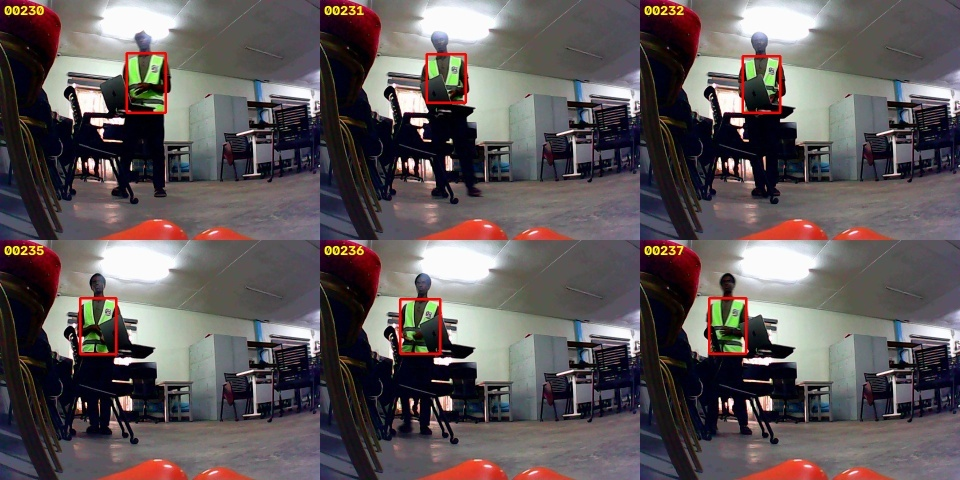
\includegraphics[width=0.62\linewidth]{figures/robot_labels.jpg}
\caption{Robot-camera frames with checked \texttt{safety\_jacket} labels (red boxes). The low viewpoint, chairs and partial views are why the original model struggled.}
\label{fig:labels}
\end{figure}

% ---------- 3. Detector ----------
\section{Detector Fine-tuning and Evaluation}
We use \textbf{YOLOv8n}~\cite{yolov8} (3.0\,M parameters), a one-stage detector small enough for real-time inference. It was fine-tuned from our original weights at 320\,px input with AdamW, a cosine learning-rate schedule and early stopping (best epoch 56 of 76, 31 minutes on an RTX~4050 laptop GPU). Inference on the GPU takes 15--20\,ms per frame.

\begin{table}[htbp]
\centering\small
\caption{Detector results on the independent test sets (320\,px). ``Found'' is the share of frames where the jacket is detected; ``false alarms'' is the share of no-vest images with any detection.}
\label{tab:det}
\begin{tabular}{l l c c c c c}
\toprule
\textbf{Test set} & \textbf{Model} & \textbf{Precision} & \textbf{Recall} & \textbf{mAP50} & \textbf{Found} & \textbf{False alarms} \\
\midrule
Robot camera (99) & Original & 0.798 & 0.777 & 0.824 & 69.1\% & 0\% \\
                  & \textbf{Fine-tuned v2} & \textbf{0.894} & \textbf{0.851} & \textbf{0.925} & \textbf{97.9\%} & 0\% \\
\midrule
Public A (242)    & Original & 0.291 & 0.193 & 0.128 & 38.2\% & 16.1\% \\
                  & Fine-tuned v1 & 0.320 & 0.159 & 0.118 & 48.4\% & 30.4\% \\
                  & \textbf{Fine-tuned v2} & \textbf{0.864} & \textbf{0.738} & \textbf{0.811} & \textbf{96.8\%} & 16.1\% \\
\midrule
Public B (208)    & Original & 0.501 & 0.345 & 0.332 & 57.1\% & 21.9\% \\
                  & Fine-tuned v1 & 0.509 & 0.325 & 0.315 & 74.1\% & 33.3\% \\
                  & \textbf{Fine-tuned v2} & \textbf{0.878} & \textbf{0.782} & \textbf{0.874} & \textbf{92.0\%} & \textbf{14.6\%} \\
\bottomrule
\end{tabular}
\end{table}

\textbf{Results (Table~\ref{tab:det}).} On the robot camera, mAP50 rose from 0.82 to 0.93 and the jacket is found in 98\% of frames instead of 69\%. On public photos of other vests, people and places the gain is much larger (mAP50 0.13$\rightarrow$0.81 and 0.33$\rightarrow$0.87), and false alarms on people without vests fell from 22\% to 15\% on set~B. A first fine-tune (v1) used only robot frames: it detected more jackets but \emph{doubled} false alarms (16$\rightarrow$30\%). This showed that negative examples are essential, and v2 adds 700 of them. Two cautions apply. The robot test frames come from the same room and day as the robot training frames, and the remaining false alarms are mostly orange or yellow clothing. We handle the latter in the follower (Section~\ref{sec:ros}).

% ---------- 4. ROS 2 ----------
\section{ROS 2 System Design}\label{sec:ros}
The system is one ROS~2 Jazzy~\cite{ros2} package, \texttt{jacket\_follower}, running on a laptop (Ubuntu 24.04 in WSL2, RTX~4050). The \textbf{same detector and follower nodes} run in Gazebo and on the real robot; only the camera source and the motor output change (Figure~\ref{fig:arch}).

\begin{figure}[htbp]
\centering
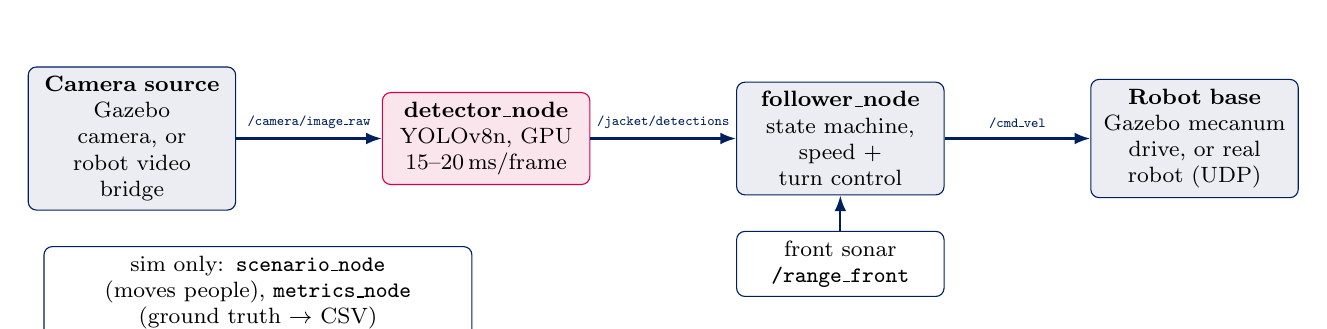
\begin{tikzpicture}[node distance=0.55cm and 1.85cm, font=\footnotesize,
  n/.style={draw=ucunavy, fill=ucunavy!8, rounded corners=3pt, align=center, minimum height=1.05cm, text width=2.4cm},
  a/.style={-{Latex[length=2mm]}, thick, ucunavy}, t/.style={font=\tiny\ttfamily, midway, above}]
  \node[n] (cam) {\textbf{Camera source}\\ Gazebo camera, or\\ robot video bridge};
  \node[n, right=of cam, fill=ucured!10, draw=ucured] (det) {\textbf{detector\_node}\\ YOLOv8n, GPU\\ 15--20\,ms/frame};
  \node[n, right=of det] (fol) {\textbf{follower\_node}\\ state machine,\\ speed + turn control};
  \node[n, right=of fol] (base) {\textbf{Robot base}\\ Gazebo mecanum drive, or real robot (UDP)};
  \draw[a] (cam) -- node[t]{/camera/image\_raw} (det);
  \draw[a] (det) -- node[t]{/jacket/detections} (fol);
  \draw[a] (fol) -- node[t]{/cmd\_vel} (base);
  \node[n, below=0.45cm of fol, minimum height=0.6cm, fill=white] (son) {front sonar \texttt{/range\_front}};
  \draw[a] (son) -- (fol);
  \node[n, below=0.45cm of cam, minimum height=0.6cm, fill=white, text width=5.2cm, xshift=1.6cm] (sim) {sim only: \texttt{scenario\_node} (moves people), \texttt{metrics\_node} (ground truth $\rightarrow$ CSV)};
\end{tikzpicture}
\caption{ROS~2 architecture. Detections are \texttt{vision\_msgs/Detection2DArray}; commands are \texttt{geometry\_msgs/Twist}.}
\label{fig:arch}
\end{figure}

\textbf{Camera input and inference.} \texttt{detector\_node} subscribes to \texttt{/camera/image\_raw} with sensor-data QoS, drops frames while busy so it never builds a backlog, crops the gripper fingertips from the bottom of real-robot images, and publishes boxes, a debug image and its inference time.

\textbf{Decision and control.} \texttt{follower\_node} runs at 20\,Hz with six states: SEARCH, CONFIRMING, FOLLOW, HOLD, TOO\_CLOSE and E\_STOP. Distance comes from the pinhole model, $d = f \cdot 0.45\,\text{m} / w_{\text{box}}$ (box width), with a second estimate from the box height and, when the target is centred, the sonar. The smallest estimate is used, because each failure mode reads too far: a side-on vest is narrow, and a close vest is cropped by the low camera. The forward speed is
\begin{equation*}
v = 0.8\,(d - 1.5) + 0.6\,\dot d, \qquad \omega = -1.6\,x_{\text{err}},
\end{equation*}
capped at 0.35\,m/s with an acceleration ramp. The $\dot d$ term reacts as soon as the gap starts to grow, so the robot \textbf{speeds up when the person speeds up}. Here $x_{\text{err}} \in [-1,1]$ is the horizontal offset of the jacket in the image.

\textbf{Uncertainty and safety.} The robot moves only after 3 consecutive detections. A \emph{new} target must score $\geq 0.70$, while the target already being followed is kept down to 0.40, and only near its last bearing. This \emph{lock-on hysteresis} stops hi-vis-coloured clothing (scored $\approx 0.55$) from capturing the robot. If the jacket is lost, the robot HOLDs for 1.5\,s, then SEARCHes by turning towards where it was last seen. It enters E\_STOP (zero velocity) if no detector output arrives for 1\,s or the sonar reads under 0.25\,m, and it never drives closer than 0.8\,m.

% ---------- 5. Gazebo ----------
\section{Gazebo Simulation}
\textbf{Setup.} Gazebo Harmonic~\cite{gazebo} with \texttt{ros\_gz\_bridge}. The MasterPi model has mecanum wheels driven by Gazebo's \texttt{MecanumDrive} plugin, with diagonal wheel friction modelling the rollers; a camera ($640\times480$ at 15\,Hz, $89^\circ$) on the arm; and a narrow front range sensor standing in for the sonar. The world is a $20\times10$\,m hall with desks. The people are textured walking-person models moved by \texttt{scenario\_node}: the worker in a hi-vis vest with silver bands, a white-shirt bystander and an orange-shirt distractor. Gazebo's odometry gives ground truth, which \texttt{metrics\_node} logs to CSV at 10\,Hz.

\textbf{Scenarios.} \textbf{S1 normal}: the worker walks 4\,m at 0.3\,m/s, turns 90$^\circ$ twice and walks back. \textbf{S2 speed}: the worker walks at 0.15, then 0.35, then 0.60\,m/s, stops, turns and walks slowly. \textbf{S3 challenging/failure}: the bystander crosses and stands between robot and worker for 20\,s while the worker turns and sprints 3.2\,m out of view at 0.8\,m/s, with the orange shirt in view. We also ran S3 with lock-on hysteresis disabled (acquire threshold 0.40) as an ablation.

\begin{table}[htbp]
\centering\small
\caption{Gazebo results (ground truth). Gap is the centre-to-centre distance while the worker walks; the closest approach is checked against the 0.8\,m stop distance.}
\label{tab:sim}
\setlength{\tabcolsep}{4pt}
\begin{tabularx}{\linewidth}{l c c c c c >{\raggedright\arraybackslash}X}
\toprule
\textbf{Scenario} & \textbf{Following} & \textbf{Wrong} & \textbf{Gap (m)} & \textbf{Closest} & \textbf{Ends on} & \textbf{Speed: worker$\rightarrow$robot (m/s)} \\
 & & \textbf{person} & & & \textbf{worker} & \\
\midrule
S1 normal walk & 95.9\% & 0\,s & 2.07$\pm$0.28 & 1.17\,m & yes & 0.30$\rightarrow$0.19 (incl.\ turns) \\
S2 speed changes & 100\% & 0\,s & 2.27$\pm$0.42 & 1.82\,m & yes & 0.15$\rightarrow$0.13, 0.35$\rightarrow$0.32, 0.60$\rightarrow$0.35 (cap) \\
S3 challenge & 69.9\% & 0\,s & 2.26$\pm$0.12 & 1.93\,m & yes & searched 27\,s, re-found the worker \\
S3, no hysteresis & 38.7\% & \textbf{11.2\,s} & 2.26$\pm$0.12 & 1.95\,m & \textbf{no} & locked onto the orange shirt \\
\bottomrule
\end{tabularx}
\end{table}

\begin{figure}[htbp]
\centering
\begin{subfigure}[b]{0.30\linewidth}\centering
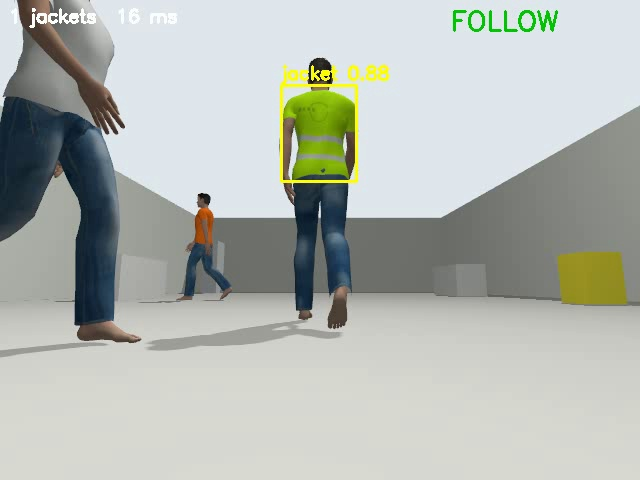
\includegraphics[width=\linewidth]{figures/sim_s3_view.jpg}
\caption{Robot camera in S3.}\end{subfigure}\hfill
\begin{subfigure}[b]{0.68\linewidth}\centering
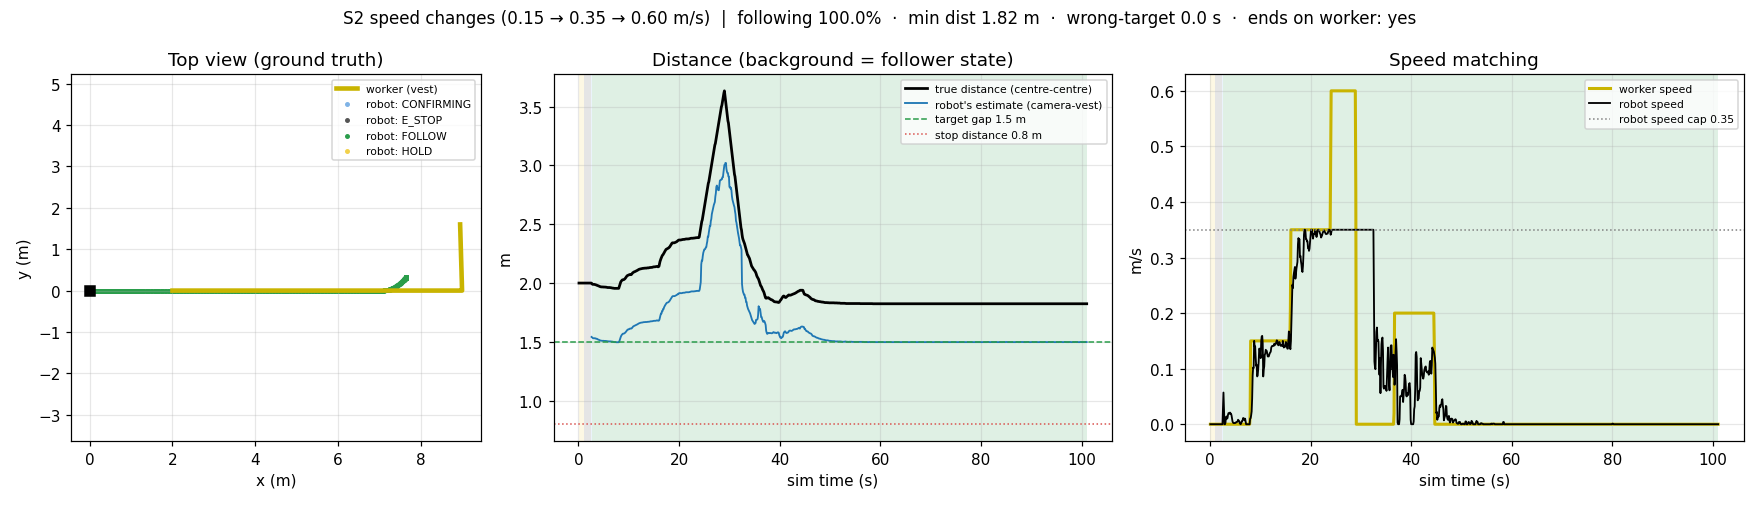
\includegraphics[width=\linewidth]{figures/sim_s2_analysis.png}
\caption{S2: top view, true vs.\ estimated distance, speeds.}\end{subfigure}
\caption{Gazebo. (a) The worker is detected (0.88) and followed while the white-shirt and orange-shirt people pass. (b) Ground truth for the speed scenario; background colours are follower states.}
\label{fig:sim}
\end{figure}

\textbf{Results (Table~\ref{tab:sim}, Figure~\ref{fig:sim}).} The robot followed the worker through both turns in S1 and never came closer than 1.17\,m. In S2 it matched the worker's speed (0.13 at 0.15\,m/s, 0.32 at 0.35\,m/s) until its 0.35\,m/s cap. At 0.60\,m/s the gap grew to 3.6\,m, but the worker stayed tracked and the robot closed the gap when they stopped. In S3 the robot lost the worker behind the bystander, searched for 27\,s, ignored the orange shirt and found the worker again. \textbf{Failure case:} without hysteresis, the robot locked onto the orange shirt and followed the wrong person for 11\,s, ending 3.7\,m from the worker. This ablation justifies the lock-on rule. Distance estimates were consistent ($\pm$0.1\,m); their 0.3--0.45\,m offset from the table's centre-to-centre ground truth is mostly geometric, since the estimate measures camera to vest surface. Detection took 16.7\,ms per frame. Building the simulation also exposed modelling bugs that we fixed: missing roller friction stopped the robot turning in place, and shared mesh textures made every person render in the vest.

% ---------- 6. Physical robot ----------
\section{Physical Deployment on the MasterPi}
The MasterPi runs Raspbian Buster with Python~3.7, which cannot run ROS~2, so we split the system. A small server on the Pi (\texttt{masterpi\_server.py}) streams the camera over HTTP and drives the mecanum wheels from UDP commands. It has its own 0.5\,s watchdog that stops the motors if commands stop, and a hard 60\% motor-power cap. On the laptop, \texttt{masterpi\_bridge} publishes the stream as \texttt{/camera/image\_raw} and sends \texttt{/cmd\_vel} to the robot, so the unchanged detector and follower nodes drive the real robot. The arm is set to a camera pose found by image-matching calibration, which also gave the camera's field of view ($\approx71^\circ$).

\textbf{Results.} With the wheels disabled, the pipeline ran at 8 frames/s with 20\,ms detection, a 10\,ms command round trip and about 30\,ms camera latency. With the wheels enabled, the robot \textbf{searched, detected the jacket (scores 0.70--0.85) and switched to FOLLOW} in three separate runs, at home and in the lab (Figure~\ref{fig:real}). It turned and drove towards the jacket, and the phone video in our demo shows it moving on its own. However, it held FOLLOW for only up to about 9\,s per run before losing the jacket, so steady following was not achieved. The causes were the hardware problems in Table~\ref{tab:challenges}.

\begin{figure}[htbp]
\centering
\begin{subfigure}[b]{0.235\linewidth}\centering
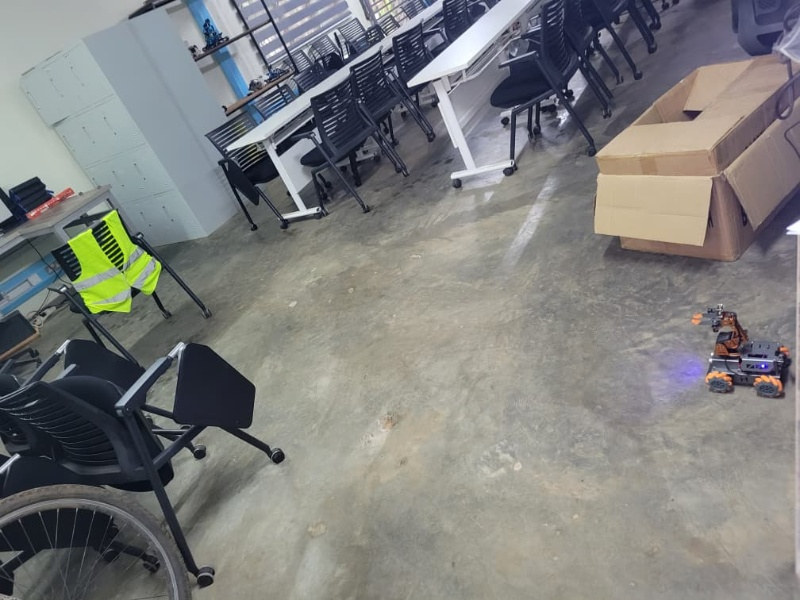
\includegraphics[width=\linewidth]{figures/robot_lab.jpg}
\caption{MasterPi in the lab.}\end{subfigure}\hfill
\begin{subfigure}[b]{0.755\linewidth}\centering
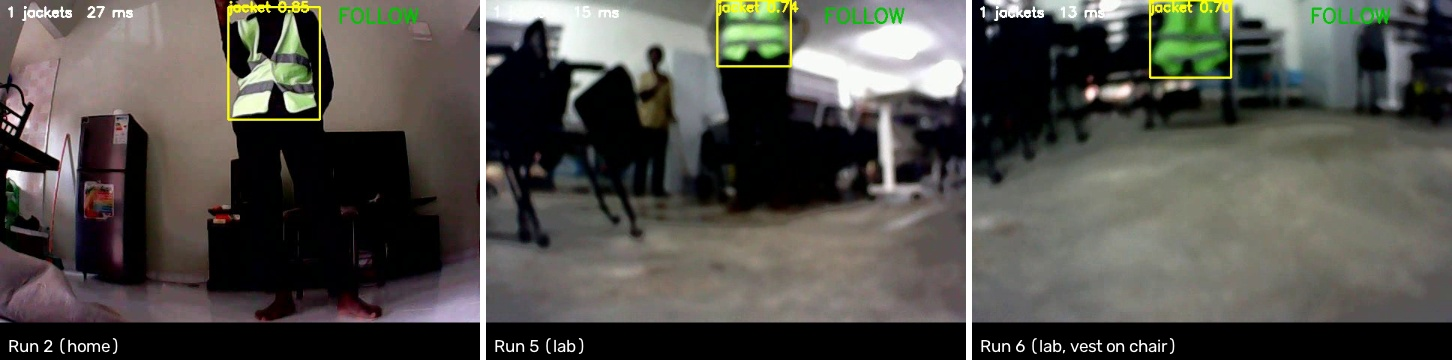
\includegraphics[width=\linewidth]{figures/real_follow_strip.jpg}
\caption{Robot view: jacket detected, state FOLLOW.}\end{subfigure}
\caption{Physical deployment: the real robot locks onto the jacket in three runs (scores 0.85, 0.74, 0.70).}
\label{fig:real}
\end{figure}

\begin{table}[htbp]
\centering\small
\caption{Challenges met on the real robot and how we handled them.}
\label{tab:challenges}
\begin{tabularx}{\linewidth}{>{\raggedright\arraybackslash}p{2.9cm} >{\raggedright\arraybackslash}X >{\raggedright\arraybackslash}X}
\toprule
\textbf{Challenge} & \textbf{What happened} & \textbf{Fix / mitigation} \\
\midrule
Unsafe motor scaling & The SDK's ``speed'' is PWM duty; our first conversion would have sent 100\% for any command & caught by reading the SDK before any wheel moved; 60\% hard cap \\
Motor dead zone & no motion below $\sim$28--32\% power, then sudden fast turns; small corrections overshoot & start-power + speed model; gentler turning on the robot \\
Battery brown-outs & the two 18650 cells sagged from 8.0 to 6.2\,V under load; the Pi rebooted mid-run & motor power scaled by battery voltage; slow, one-servo-at-a-time arm moves \\
Runaway after reboot & the motor board kept its last speed when the Pi rebooted, so the robot spun until stopped remotely & a boot service zeroes all motors at start-up (the watchdog lives on the Pi, so it cannot cover a reboot) \\
Camera blur and dim light & out of focus; 1.5 frames/s at $640\times480$; a jacket on a chair at 3\,m was not detected at all & manual focus, MJPG mode (8.5 frames/s), camera tilt; lock-on threshold 0.50 on the robot \\
Frame rate while driving & 2--3 frames/s under motor load on a weak battery, so the robot reacts late & 2\,s watchdog, stop-and-look search (turn, pause, look) \\
Wi-Fi drops & the laptop silently left the robot's hotspot (no internet) & auto-reconnect; the robot stops itself when commands stop \\
\bottomrule
\end{tabularx}
\end{table}

% ---------- 7. Discussion ----------
\section{Discussion and Limitations}
Fine-tuning with deployment-view data \emph{and} negatives was the key to a usable detector. Ground-truth evaluation in Gazebo showed the follower design works: it follows, matches speed up to the robot's limit, recovers from occlusion and, thanks to hysteresis, does not switch to a look-alike. The real robot showed what simulation hides. Power, light and actuators limited performance more than the algorithms did, and several safety mechanisms, such as the boot-time motor stop, were only discovered on hardware. Limitations: the robot test set is from one room and day; the 0.35\,m/s cap means the robot falls behind faster walkers; a person closer than about 1\,m is outside the low camera's view; detection range drops in dim light; and the real-robot results are a few short runs, not a measured benchmark.

\textbf{Future work.} Fresh batteries and a repeat of the following test, with ground truth from a tape-marked course; a test set from a new location and lighting; pan-servo tracking so the camera keeps the jacket in view while the chassis turns; a camera with better low-light exposure; and running the detector on the robot itself (ONNX or TFLite) to remove the Wi-Fi dependency.

% ---------- 8. Conclusion ----------
\section{Conclusion}
We fine-tuned a YOLOv8n safety-jacket detector (robot-camera mAP50 0.82$\rightarrow$0.93, jacket found in 98\% of frames) and built a ROS~2 follower with distance-based speed matching, search and fail-safe states. In Gazebo the robot followed the worker in all three scenarios, and our ablation showed that lock-on hysteresis prevents following the wrong person. On the physical MasterPi the full pipeline is deployed and the robot detects and locks onto the jacket. Steady real-world following is limited by the battery, camera and motors, and these are our next steps.

% ---------- 9. Contributions ----------
\section{Individual Contributions}
\begin{tabularx}{\linewidth}{>{\raggedright\arraybackslash}p{3.6cm} X}
\toprule
\textbf{Jamugisa Peter Paul} (S25M25/008) & Detector: robot-camera data collection, Grounding DINO auto-labelling and checking, dataset building, fine-tuning v1/v2 and independent evaluation. Physical deployment: robot server, ROS~2 bridge, camera and motor calibration, safety fixes and live robot tests. \\
\textbf{Ayebare Moses} (S25M25/003) & ROS~2 package: detector, follower, bridge, scenario and metrics nodes, launch files and parameters. Gazebo: MasterPi model, hall world, people models, the three scenarios, ground-truth metrics and simulation evaluation. \\
\bottomrule
\end{tabularx}

\small
\begin{thebibliography}{9}\setlength{\itemsep}{0pt}
\bibitem{yolov8} G.~Jocher, A.~Chaurasia and J.~Qiu, \emph{Ultralytics YOLOv8}, 2023. \url{https://github.com/ultralytics/ultralytics}
\bibitem{gdino} S.~Liu \emph{et al.}, ``Grounding DINO: Marrying DINO with grounded pre-training for open-set object detection,'' arXiv:2303.05499, 2023.
\bibitem{hb1204} HB1204, \emph{PPE\_Detection} dataset (Roboflow export, CC BY 4.0), Hugging Face, 2024.
\bibitem{vincent} V.~Gourbin, \emph{ppe-detection} dataset (Roboflow export, CC BY 4.0), Hugging Face, 2024.
\bibitem{ros2} S.~Macenski \emph{et al.}, ``Robot Operating System 2: Design, architecture, and uses in the wild,'' \emph{Science Robotics}, 7(66), 2022.
\bibitem{gazebo} Open Robotics, \emph{Gazebo Harmonic}, \url{https://gazebosim.org}, 2023.
\bibitem{masterpi} Hiwonder, \emph{MasterPi documentation}, \url{https://docs.hiwonder.com/projects/MasterPi}.
\end{thebibliography}

\end{document}
